\chapter{ОЗНАКОМЛЕНИЕ С НАБОРОМ TETRIX}
<<TETRIX>> предоставляет идеальную платформу для создания гибкого
и творческого проекта робота. На ее основе можно построить робота
с дистанционным управлением или, используя микрокомпьютер
и датчики, создать автономного робота. Состав данного набора
представлен на рисунке \ref{fig:all}.
Это робототехнический конструктор
нового поколения, который позволяет перевести процесс создания робота
на новый качественный уровень с практически неограниченными возможностями.
\\
\begin{figure}[hb]
    \centering
    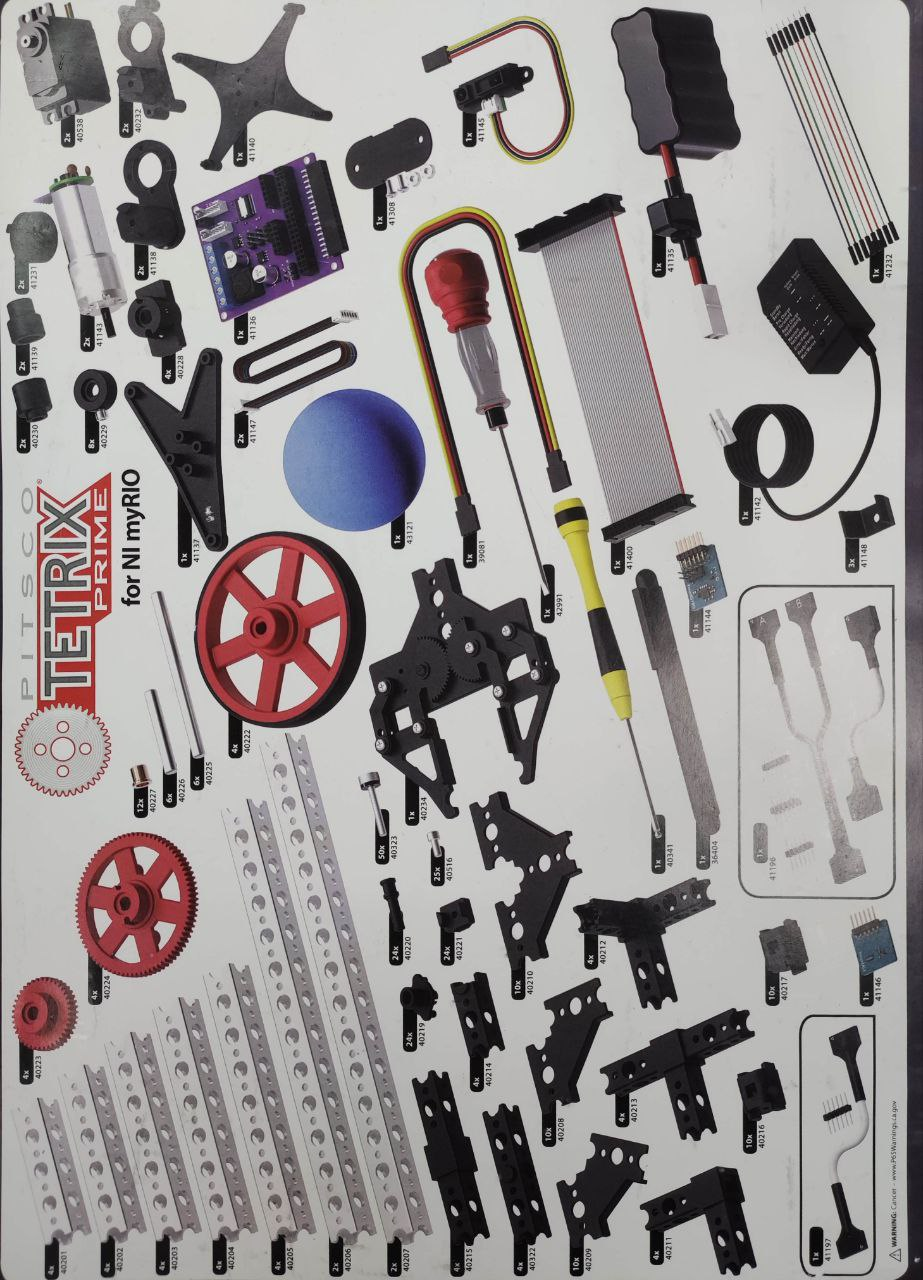
\includegraphics[scale=0.35]{fig/2.1.jpg}
    \caption{Состав робототехнического набора <<TETRIX>>}
    \label{fig:all}
\end{figure}

\section{Советы по сборке и наладке к робототехническому набору}
Если заранее продумать удобный доступ к крепежу, то у всех, кто участвует в сборке, останутся положительные впечатления.
Как правило, при создании какого-либо промежуточного узла разумно лишь наживлять гайки и болты, пока не будет уверенности,
что все детали находятся на положенном им месте. Затем дозатяните весь крепёж перед следующим шагом.\cite{3}

\subsection{Размещение профильных реек}
Если немного спланировать свои действия и предварительно обдумать, как лучше соединить конструктивные элементы, то сборка
пойдёт легче, быстрее и успешнее.\cite{1}

\begin{figure}[h]
    \centering
    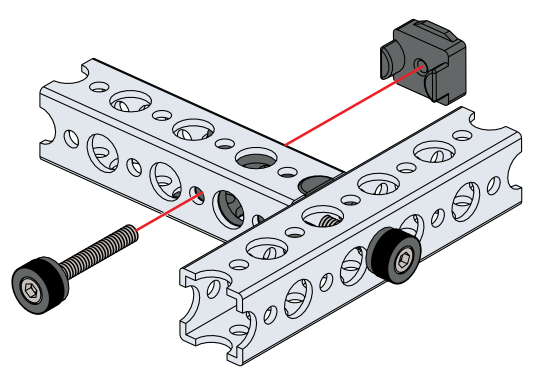
\includegraphics[scale=0.4]{fig/2.2.png}
    \caption{Размещение профильных реек с предварительным анализом сборки}
    \label{fig:razm}
\end{figure}

На рисунке \ref{fig:razm} у обеих конструкций одинаковые монтажные поверхности, но привинчивать зубчатые гайки не одинаково
удобно. Вариант с удобным доступом к крепежу предпочтительнее. По возможности избегайте положений, затрудняющих
доступ к крепёжным деталям.

\subsection{Использование инструментов}
Правильное использование простейших инструментов (рисунок \ref{fig:inst}) упрощает сборку, делает её приятнее и экономит время.

\subsection{Использование выгодных особенностей конструкции}
Конструктивные особенности некоторых деталей усиливают их полезность или имеют особое назначение. Если знать и применять
эти особенности в полной мере, то собранная модель получится прочнее, долговечнее и работать будет лучше.\cite{2}

Это правильное положение зубчатых гаек. Самостопорящейся стороной зубчатая гайка должна всегда быть обращена к гладкой
стороне конструктивного элемента, пример продемонстрирован на рисунке \ref{fig:const}.

\begin{figure}[h]
    \centering
    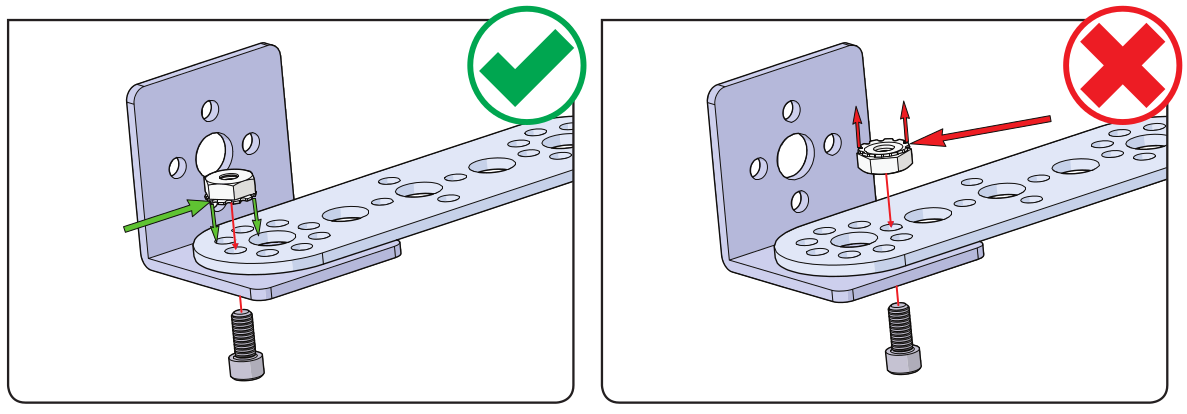
\includegraphics[scale=0.3]{fig/2.4.png}
    \caption{Использование выгодных особенностей конструкции}
    \label{fig:const}
\end{figure}

\begin{figure}[h]
    \centering
    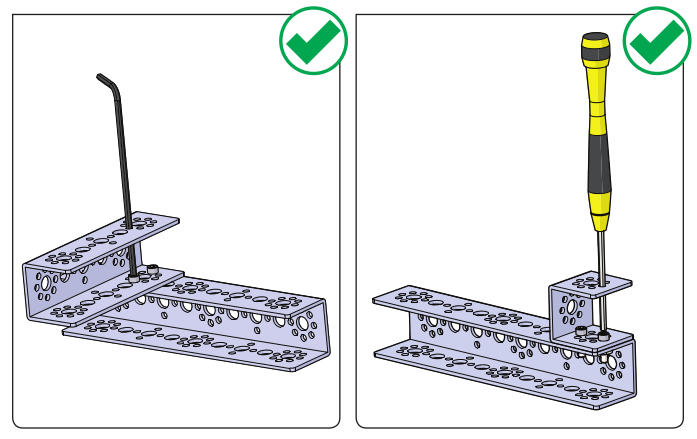
\includegraphics[scale=0.5]{fig/2.3.png}
    \caption{Правильное использование инструментов}
    \label{fig:inst}
\end{figure}

